\documentclass[tikz, border=1mm]{standalone}
\usepackage[T1]{fontenc}
\usepackage{lmodern}

\definecolor{pCyan}{RGB}{149,186,201}

% Cylindric tableau with m=3 rows per period and shift ell=2, after
% Alexandersson--Kantarci Oguz, "Cylindric Schur functions", Example 27
% (redrawn in English notation).  Row r occupies y in [-r,-r+1] and
% column c occupies x in [c-1,c].  Rows 1--3 are the fundamental domain;
% row r+3 is row r shifted two columns to the left.
\newcommand{\cell}[4]{% #1 row, #2 column, #3 entry, #4 style
  \draw[#4] (#2-1,-#1) rectangle (#2,-#1+1);
  \node at (#2-0.5,-#1+0.5) {#3};}

\begin{document}
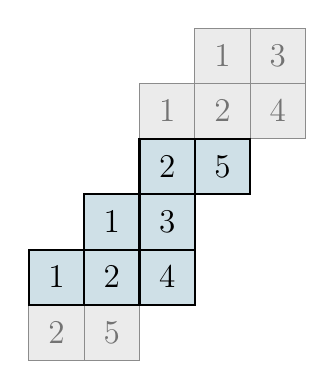
\begin{tikzpicture}[x=2em, y=2em, every node/.style={font=\large}]
  \tikzset{main/.style={fill=pCyan!45, draw=black, thick},
           copy/.style={fill=black!8, draw=black!45}}
  % Copies of the fundamental domain (gray).
  \begin{scope}[every node/.append style={text=black!55}]
    \cell{-1}{4}{1}{copy} \cell{-1}{5}{3}{copy}
    \cell{0}{3}{1}{copy} \cell{0}{4}{2}{copy} \cell{0}{5}{4}{copy}
    \cell{4}{1}{2}{copy} \cell{4}{2}{5}{copy}
  \end{scope}
  % Fundamental domain: rows 1, 2, 3.
  \cell{1}{3}{2}{main} \cell{1}{4}{5}{main}
  \cell{2}{2}{1}{main} \cell{2}{3}{3}{main}
  \cell{3}{1}{1}{main} \cell{3}{2}{2}{main} \cell{3}{3}{4}{main}
\end{tikzpicture}
\end{document}
